\subsection{Arquitectura de los Componentes del Sistema}\label{subsec:arquitectura}

Más allá de la elección del \textit{stack} tecnológico, la calidad a largo plazo de un sistema depende de las decisiones de diseño que gobiernan la organización interna de su código. En \texttt{paralegales-ui} y \texttt{paralegales-services}, estas decisiones se concretaron mediante la adopción y refactorización de patrones arquitectónicos deliberados —uno en la capa \textit{frontend} y otro en la capa \textit{backend}—, con el objetivo compartido de mejorar la mantenibilidad, la testabilidad y la capacidad de evolución independiente de cada componente.

\subsubsection{Capa \textit{Frontend}: Nuxt~3, Domain-Driven Design y Nuxt Layers}

La arquitectura de \texttt{paralegales-ui} fue diseñada con una perspectiva de escalabilidad y mantenibilidad a largo plazo. Basada en los principios de \textit{Domain-Driven Design} (DDD), la aplicación implementa una estructura modular mediante Nuxt Layers, mecanismo que permite que cada dominio funcional constituya una unidad autónoma y componible. Integrando tanto el tema visual aislado como cada dominio de negocio como una capa independiente. El proyecto se compone de nueve \textit{features}: autenticación, gestión de procesos, pagos, detalle de procesos, búsqueda, configuración de usuario, seguimiento activo, \textit{landing page} y términos y condiciones.

La aplicación está organizada en cuatro niveles de abstracción, cuyos límites de responsabilidad son explícitos y estables:

\begin{enumerate}
  \item \textbf{Capa de aplicación (\texttt{app-core/}):} aloja los componentes de infraestructura global del sistema, tales como \textit{layouts}, \textit{middleware}, navegación y \textit{plugins}. Estas son responsabilidades transversales a todos los dominios y se configuran de manera centralizada.

  \item \textbf{Capa compartida (\texttt{common/}):} contiene \textit{composables} reutilizables, utilidades, componentes genéricos, modelos de dominio compartidos y la configuración de los clientes HTTP (\texttt{\$apiClientParalegalesBackend} y \texttt{\$apiClientInternal}). Esta capa representa el \textit{shared kernel} del DDD: elementos que múltiples \textit{features} reutilizan sin depender de un dominio específico. Aquí también reside el BFF implementado en \texttt{common/server/utils}, que gestiona llamadas complejas o sensibles hacia el \textit{backend} de Paralegales desde el lado del servidor.

  \item \textbf{Capas de \textit{features} (\texttt{features/}):} cada \textit{feature} es un \textit{bounded context} en términos de DDD. Por ejemplo, la \textit{feature} \texttt{auth} engloba la autenticación en su totalidad (componentes, servicios, \textit{composables}, páginas y utilidades específicas); \texttt{payments} aglutina toda la lógica de compra y renovación de planes; \texttt{my-processes} centraliza la consulta y gestión de procesos del usuario. Cada \textit{feature} posee su propio \texttt{nuxt.config.ts} que declara sus componentes locales y dependencias específicas, lo que permite modificarla, probarla o reemplazarla de forma totalmente independiente.

  \item \textbf{Capa de tema (\texttt{vendor/vuexy/}):} completamente aislada, contiene la biblioteca de interfaz de usuario Vuexy, sus estilos, componentes temáticos y configuración de diseño. Esta separación garantiza que el tema pueda actualizarse o reemplazarse sin afectar la lógica de dominio, evitando que detalles de implementación visual contaminen las capas funcionales.
\end{enumerate}

La configuración de Nuxt integra \textit{auto-imports} para reducir la verbosidad en el desarrollo: \textit{composables}, utilidades y \textit{stores} de \texttt{common/} están disponibles globalmente sin importaciones explícitas. El estado global se centraliza en \textit{stores} de Pinia alojadas en \texttt{common/stores/}, permitiendo que \textit{features} independientes compartan información de forma controlada sin acoplamiento directo entre ellas. Los beneficios de esta arquitectura son directamente observables: nuevas \textit{features} se incorporan sin riesgo de conflicto con el código existente; cambios en un dominio no requieren análisis de impacto sobre el resto del proyecto; y el aislamiento del tema permite actualizar la biblioteca de UI sin riesgo de ruptura en la lógica de negocio.

\subsubsection{Capa \textit{Backend}: Patrón Handler, Service y Repository}

La capa de servicios en \texttt{paralegales-services} fue refactorizada para adoptar una separación clara de responsabilidades mediante el patrón \textbf{Handler -- Service Struct -- Abstract Repository}. Este diseño fue motivado originalmente por una estrategia de migración de base de datos (de Firestore hacia AWS DynamoDB), aunque dicha migración no se concretó finalmente por decisiones de producto y empresa. El patrón resultante, no obstante, aportó beneficios inmediatos de legibilidad, testabilidad y mantenibilidad que justifican su adopción con independencia del caso de uso de migración.

Cada función Lambda del sistema consta típicamente de tres componentes diferenciados:

\begin{enumerate}
  \item \textbf{Handler (\texttt{main.go}):} punto de entrada de la función AWS Lambda. Es responsable de deserializar el evento de entrada —por ejemplo, un mensaje SQS—, inicializar las dependencias (como el cliente Firestore) e invocar la lógica de negocio. Su implementación es deliberadamente delgada, delegando toda la orquestación al \textit{service}.

  \item \textbf{Service Struct (\texttt{service.go}):} contiene toda la lógica de negocio de la función. Recibe el repositorio como dependencia inyectada, lo que le permite operar de forma agnóstica respecto a la tecnología de persistencia subyacente. Su responsabilidad es orquestar las operaciones: consultar información, procesar cambios, actualizar registros, publicar eventos en colas, etcétera.

  \item \textbf{Abstracción del repositorio (\texttt{repository\_interface.go} + \texttt{repository\_firestore.go}):} define una interfaz genérica que especifica las operaciones de persistencia (lectura, escritura y consultas). Una implementación concreta —como \texttt{FirestoreCheckProcessesRepository}— realiza las operaciones reales contra Firestore. Esta abstracción constituye el núcleo de la flexibilidad arquitectónica del componente.
\end{enumerate}

El flujo de ejecución sigue la cadena: el \textit{Handler} instancia la implementación concreta del repositorio, instancia el \textit{Service} inyectando dicho repositorio, e invoca \texttt{Service.Run()}, que ejecuta la lógica de negocio a través de los métodos del repositorio. Tal como se aprecia en la \autoref{fig:api-gateway}, las funciones Lambda quedan expuestas de forma unificada a través de Amazon API Gateway, que actúa como punto de entrada único para las peticiones provenientes del BFF. Este diseño permite escribir pruebas unitarias sin acceder a la base de datos real: al inyectar una implementación \textit{mock} del repositorio, los \textit{tests} validan la lógica del \textit{service} de forma rápida y determinística, sin latencia de entrada/salida ni efectos secundarios sobre datos reales. Asimismo, si en el futuro se requiere cambiar de proveedor de persistencia, bastará con crear una nueva implementación del repositorio que cumpla el mismo contrato de interfaz —por ejemplo, \texttt{DynamoDBCheckProcessesRepository}—, sin modificar una sola línea del \textit{service}.

\newcommand\apiGatewayCaption{Integración de las funciones Lambda del \textit{backend} con Amazon API Gateway. \hspace{1em}}
\begin{figure}[H]
  \centering
  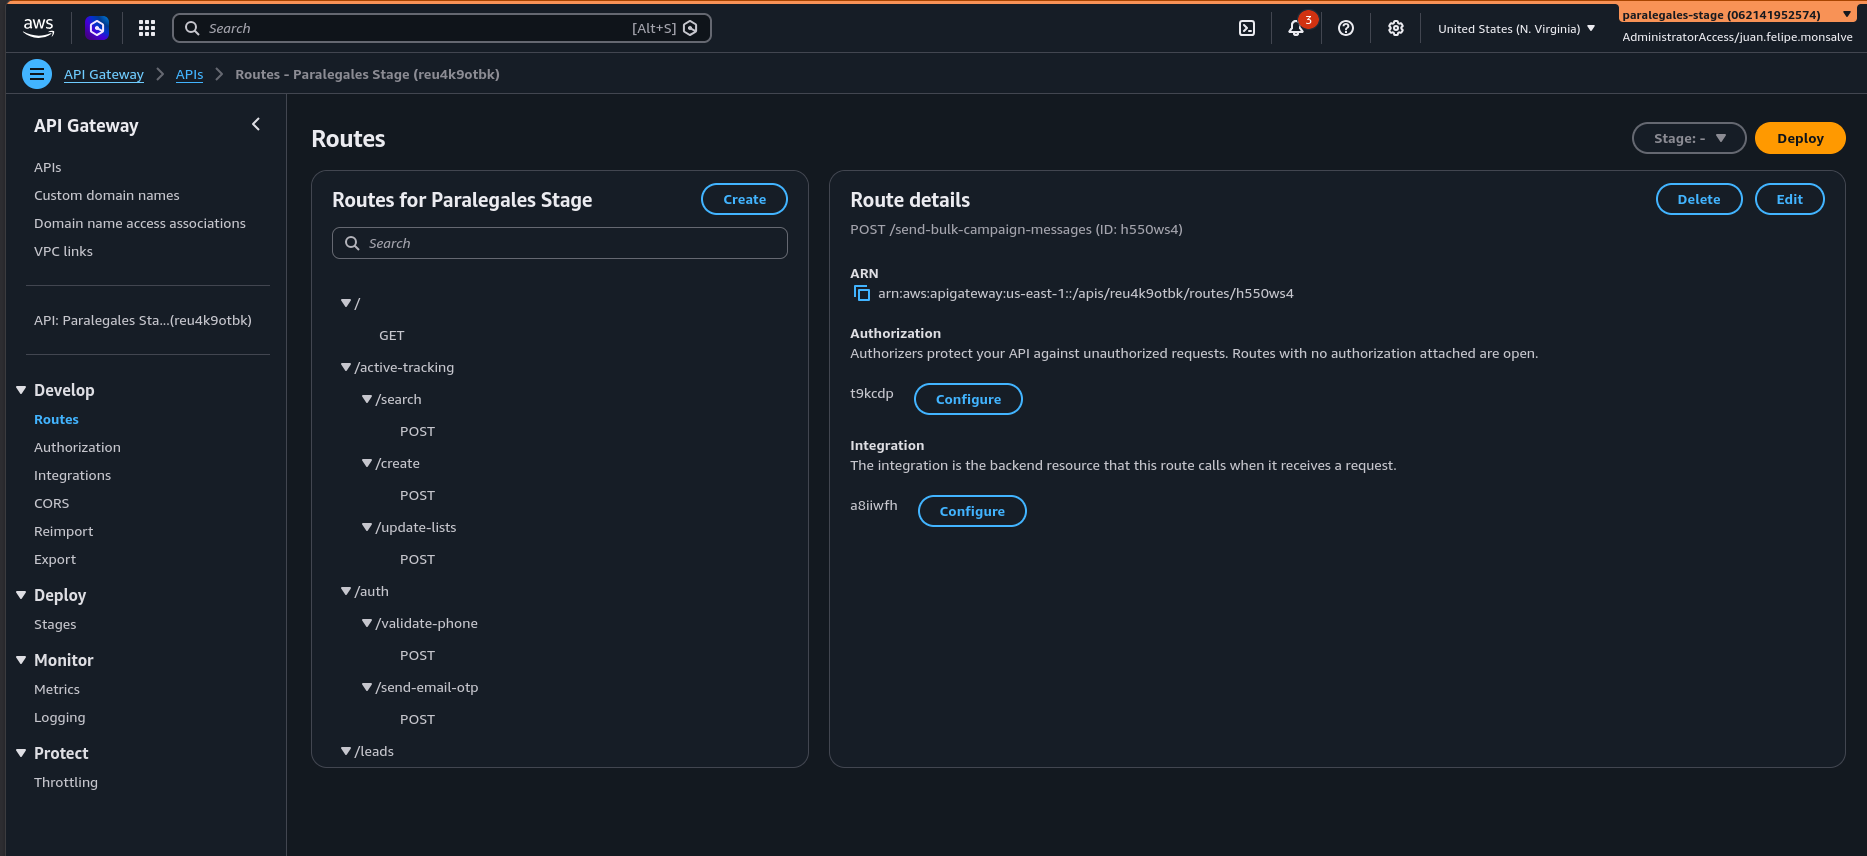
\includegraphics[width=1\textwidth]{img/figures/fig14-api-gateway.png}
  \caption[\apiGatewayCaption]{\apiGatewayCaption Fuente: Elaboración propia.}
  \label{fig:api-gateway}
\end{figure}

La capa de persistencia del sistema está respaldada por Firestore, base de datos documental de Firebase. Tal como ilustra la \autoref{fig:base-datos-firestore}, la organización de las colecciones refleja directamente los dominios de negocio de la plataforma: usuarios, procesos, seguimientos activos y planes de suscripción, entre otros. Esta estructura documental facilita la consulta eficiente de datos jerárquicos y la sincronización en tiempo real, características especialmente valiosas para los flujos reactivos implementados en el \textit{frontend}.

\newcommand\basesDatosFirestoreCaption{Estructura de colecciones y documentos en la base de datos Firestore. \hspace{1em}}
\begin{figure}[H]
  \centering
  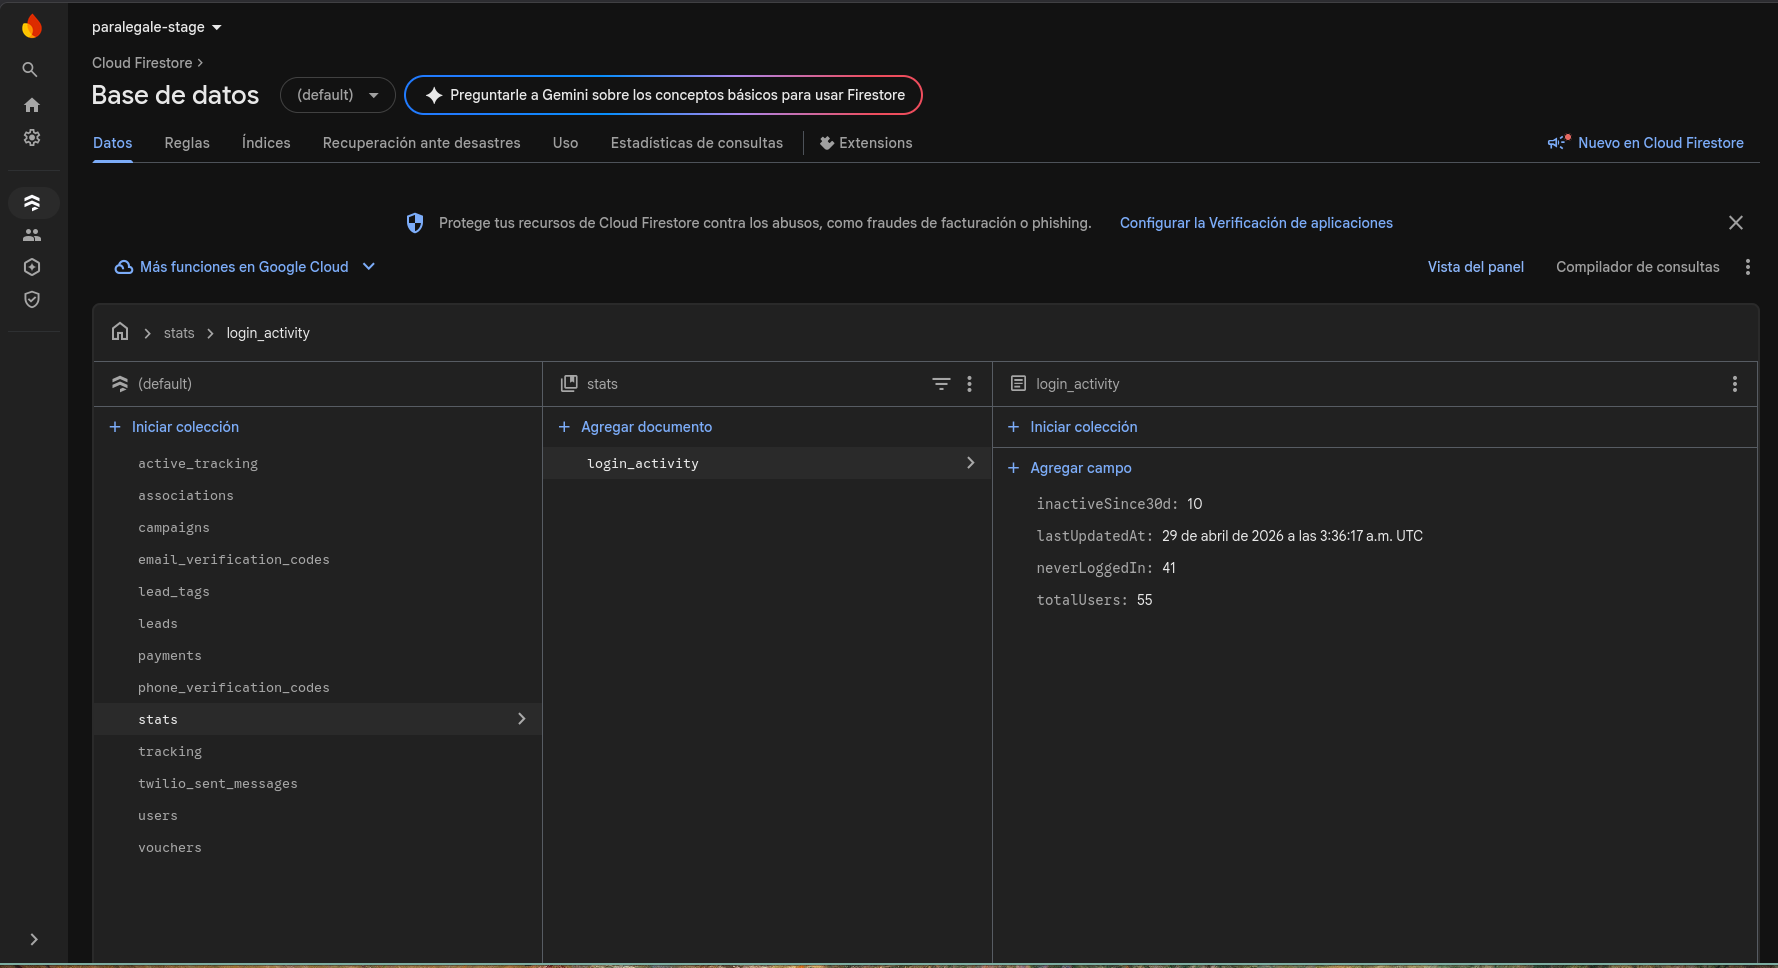
\includegraphics[width=1\textwidth]{img/figures/fig14-base-datos-firestore.png}
  \caption[\basesDatosFirestoreCaption]{\basesDatosFirestoreCaption Fuente: Elaboración propia.}
  \label{fig:base-datos-firestore}
\end{figure}

Establecidos los fundamentos tecnológicos y la organización arquitectónica del sistema, los siguientes apartados describen los módulos funcionales que dan forma a las capacidades de negocio de Paralegales, comenzando por el módulo transversal que regula el acceso a toda la plataforma: la autenticación.
